\scanpage{340}
% R340.01 | text | top, lines 1--12 | Ce calcul suggère fortement
Ce calcul suggère fortement que les relations \unsure{par|en} (64) impliquent déjà (68)\ldots{} c'est $\unsure{\overline{\mathrm m}}$ à peu de choses près une démonstration\ldots{} Si on admet ce point, il reste seulement à vérifier que les conditions précédentes \inserted{(64)} (i.e. essentiellement déjà (51) à (56) sauf (55)) impliquent aussi (55), i.e. l'indépendance des $\varepsilon_0,\varepsilon_1$ en toute fibre, i.e. que $N_0,N_1$ sont non-homothétiques en \unsure{tte} fibre. Or (67)
% R340.02 | display | upper middle, line 13 | N_1=tilde sigma(N_0)
\[
(*)\qquad N_1=\widetilde\sigma(N_0),\ \unsure{\deleted{\text{et}}}\ \inserted{=\widetilde\rho(\unsure{N_1|N_0})}\ \deleted{N_0=\unsure{\widetilde\sigma(N_1)}}\,\unsure{:}
\]
% R340.03 | text | middle, line 14 | Si on avait sur une fibre
Si on avait sur une fibre
% R340.04 | display | middle, line 15 | N_1=lambda N_0
\[
\unsure{(\deleted{74})}\qquad N_1=\lambda N_0
\]
% R340.05 | text | middle, lines 16--18 | on en conclurait
on en conclurait, en \unsure{appliquant} \deleted{$\widetilde\sigma$ et} utilisant $\widetilde\sigma^2=1$, \inserted{et $\widetilde\rho^3=1$,} \inserted{les relations} \deleted{$\widetilde\sigma(N_1)=N_0$, $\widetilde\sigma(N_0)=N_1$}
% R340.06 | display | lower middle, lines 19--20 | N_0=lambda N_1
\[
\deleted{\unsure{(**)}\qquad
\left\{\begin{aligned}
N_0&=\lambda N_1\unsure{\deleted{=\lambda^2}},\quad
\text{donc }\deleted{\lambda^2=1}\ N_0=\lambda^2N_0\quad\text{d'où}\\
\lambda^2&=1.
\end{aligned}\right.}
\]
% R340.07 | text | lower middle, line 21 | Mais un calcul immédiat
\deleted{Mais un calcul immédiat donne aussi}
% R340.08 | display | lower middle, line 22 | N_0=rho^{-1}N
\[
\deleted{(**)\qquad N_0=\rho^{-1}N,\quad N_1\unsure{.}}
\]
% R340.09 | display | lower, line 23 | lambda^2=1,lambda^3=1
\[
\lambda^2=1,\quad\lambda^3=1\qquad\text{d'où }\lambda=1
\]
% R340.10 | text | lower, lines 24--28 | i.e. N_0=N_1
i.e. $N_0=N_1$ i.e. $N_0$ commute à $\sigma,\rho$ donc aussi $N=-\sigma N_0$ \inserted{$=\rho^{-1}N_0$} commute à $\sigma,\rho$, et comme $N=\sigma+\rho$, $\sigma$ et $\rho$ commutent. Mais alors
% R340.11 | text | bottom left | 339
\mspage{339}

\scanpage{341}
% R341.01 | text | top centre | 471
\mspage{471}
% R341.02 | display | top, lines 1--2 | (sigma+rho)^2
\[
(\sigma+\rho)^2=\underbrace{\sigma^2}_{-1}+\underbrace{\rho^2}_{\rho-1}+2\sigma\rho=\rho-2+2\sigma\rho=
\]
% R341.03 | text | upper, line 3 | donc la relation
donc la relation $(\sigma+\rho)^2=\sigma+\rho$ s'écrit
% R341.04 | display | upper, lines 4--5 | rho-2+2 sigma rho
\[
\deleted{\rho}-2+2\sigma\rho=\sigma+\deleted{\rho}\qquad\text{i.e.}
\]
\[
\deleted{\unsure{(**)}}\qquad
2\sigma\rho=\sigma+2\quad\text{soit}\quad
\underbrace{2\sigma^2\rho}_{-2\rho}=\underbrace{\sigma^2}_{-1}+2\sigma
\quad\text{i.e.}\quad 2(\sigma+\rho)=1
\]
% R341.05 | text | upper middle, lines 6--14 | Prenant les traces
\deleted{Prenant les traces des deux mbs, et utilisant $\operatorname{Tr}\sigma\rho=2$ (74), $\operatorname{Tr}\sigma=0$, $\operatorname{Tr}1=2$, on trouve $4=4$, pas de contradiction mais prenant les déterminants \inserted{des deux mbs de \unsure{(**)},} on trouve (\deleted{\unsure{det}} admettant que $\det\sigma=\det\rho=1$, ce qui est une conséquence de (64) pour peu qu'on exige de plus que $\sigma,\rho$ soient réguliers i.e. ne soient des scalaires sur aucune fibre) on trouve}
% R341.06 | margin note | left of lines 12--14 | double vertical stroke
\margin{$\Vert$}
% R341.07 | display | middle, line 15 | 2^2=2^2+2 Tr sigma
\[
\deleted{(***)\qquad 2^2=2^2+2\underbrace{\operatorname{Tr}\sigma}_{0}+\underbrace{(\det\sigma)^{\unsure{2}}}_{1}\quad\text{i.e.}\quad 1=0}
\]
% R341.08 | text | middle, lines 16--17 | ce qui est absurde
\deleted{ce qui est absurde. d'où, en prenant}

\deleted{Je \unsure{le} \unsure{ve.}}
% R341.09 | display | lower middle, line 18 | 2N=1
\[
(**)\qquad 2N=1,
\]
% R341.10 | text | lower middle, line 19 | d'où, en prenant
d'où, en prenant les déterminants
% R341.11 | display | lower middle, line 20 | 4 det N=1
\[
4\underbrace{\det N}_{0}=1\qquad\text{i.e.}\quad 0=1,\quad\text{\uline{absurde}.}
\]
% R341.12 | text | lower, lines 21--25 | Remarque Je ne serais pas étonné
\deleted{Je ne \unsure{serais|sera}}

\uline{Remarque} Je ne serais pas étonné qu'on ait aussi des conditions équivalentes à (51) à (56) sous la forme
% R341.13 | display | bottom, line 26 | (75) sigma^2+1
\[
(75)\qquad \sigma^2+1=\rho^{\unsure{3|2}}\unsure{-|+}\rho+1=0,\quad
\varepsilon_0\mathrel{\overset{\mathrm{dfn}}{=}}-\sigma^{-1}\rho\ \text{est unipotent régulier}
\]
% R341.14 | text | bottom left | 340
\mspage{340}

\scanpage{342}
% R342.01 | text | top, lines 1--4 | en exigeant de plus
en exigeant de plus, au besoin, que $\sigma,\rho$ soient également réguliers i.e. ne soient des scalaires sur aucune fibre. Il faudrait se convaincre que cela implique que
% R342.02 | display | upper, line 5 | N=dfn rho+sigma
\[
N\mathrel{\overset{\mathrm{dfn}}{=}}\rho+\sigma
\]
% R342.03 | text | upper, line 6 | satisfait bien la relation
satisfait bien la relation d'idempotence
% R342.04 | display | upper, line 7 | N^2-N=0
\[
\unsure{(75)|(76)}\qquad N^2-N=0
\]
% R342.05 | text | upper middle, line 8 | ce qui équivaut
(ce qui équivaut, si $N$ régulier, à
% R342.06 | display | upper middle, line 9 | Tr N=1,det N=0
\[
(77)\qquad \operatorname{Tr}N=1,\quad\det N=0\qquad (?)
\]
% R342.07 | text | middle, lines 10--13 | Mais N est régulier
Mais $N$ est régulier, car si sur une fibre \unsure{c'était} un scalaire on aurait que (en se restreignant à cette fibre) $\rho$ et $\sigma$ commutent, on aurait
% R342.08 | display | middle, lines 14--15 | -sigma^{-1}rho=sigma rho
\[
\begin{aligned}
-\sigma^{-1}\rho&=\sigma\rho=\varepsilon_0=1+N_0\\
-\inserted{\unsure{''}}\rho\sigma^{-1}&=\rho\sigma=\varepsilon_1=1+N_1,
\end{aligned}
\]
% R342.09 | deletion | middle, beneath second epsilon identity | Prenant
\deleted{\unsure{Prenant} $\unsure{\varepsilon_0=\det\rho}$}

\deleted{avec}
% R342.10 | display | middle-lower, lines 16--18 | (1-sigma rho)^2=0
\[
(1-\sigma\rho)^2=0\quad\text{i.e.}\quad
1-2\sigma\rho+\underbrace{\sigma^2}_{-1}\underbrace{\rho^2}_{\rho-1}=0\quad\text{i.e.}
\]
\[
1-2\sigma\rho+1-\rho=0\quad\text{i.e.}\quad 2=\rho+2\sigma\rho
\]
% R342.11 | text | lower, line 19 | soit, en multipliant
soit, en multipliant par $\sigma$
% R342.12 | display | lower, line 20 | 2 sigma=rho sigma+2 sigma^2 rho
\[
2\sigma\unsure{=}\rho\sigma+2\underbrace{\sigma^2}_{-1}\rho
\quad\text{i.e.}\quad 2\underbrace{(\sigma+\rho)}_{N}=\rho\sigma
\]
% R342.13 | text | lower, lines 21--23 | Mais par hyp.
Mais par hyp. on a $N=\lambda.1$, $\lambda$ scalaire, d'où $\rho\sigma=2\lambda$, et prenant les déterminants
% R342.14 | display | lower, line 24 | det(rho sigma)=4 lambda^2
\[
\det\underbrace{(\rho\sigma)}_{1}=4\lambda^2
\]
% R342.15 | text | bottom, line 25 | i.e. 2 inv.
i.e. $\deleted{\unsure{4}}\ 2$ inv. et $\lambda=\dfrac{\varepsilon}{2}$, avec $\varepsilon^2=1$,
% R342.16 | display | bottom, lines 26--27 | rho sigma=epsilon
\[
\begin{aligned}
\text{i.e.}\qquad&\rho\sigma=\varepsilon\qquad\varepsilon^2=1,\\
&\rho^2\underbrace{\sigma^2}_{-1}=1\qquad\underbrace{\rho^2}_{\rho-1}=-1,\quad\text{i.e.}\quad\rho=0,\quad\text{\uline{absurde}}
\end{aligned}
\]
% R342.17 | text | bottom left | 341
\mspage{341}

\scanpage{343}
% R343.01 | text | top centre | 472
\mspage{472}
% R343.02 | deletion | top, line 1 | Mais Tr N=0
\deleted{Mais $\operatorname{Tr}N=0$ \unsure{par}}
% R343.03 | text | upper, lines 2--4 | Donc N est régulier
Donc $N$ est régulier, il reste à prouver (77).

Mais $\operatorname{Tr}N=\underbrace{\operatorname{Tr}\sigma}_{0}+\underbrace{\operatorname{Tr}\rho}_{1}=1$, OK, reste à prouver $\det(\rho+\sigma)=0$ mais
% R343.04 | display | upper middle, line 5 | det(rho+sigma)
\margin{\figure{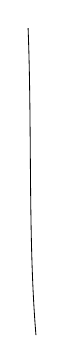
\begin{tikzpicture}[x=1mm,y=1mm]\draw[line width=.3pt] (1,0) .. controls (0,12) and (.5,26) .. (0,39);\end{tikzpicture}}}
\[
\det(\rho+\sigma)=\deleted{\underbrace{\det\rho}_{1}+\underbrace{\det\sigma}_{1}+\operatorname{Tr}(\sigma\rho)}
\]
% R343.05 | deletion | upper middle, lines 5--6 | et la relation équivaut
\deleted{et la relation équivaut}
% R343.06 | display | middle, lines 6--9 | det sigma(1+sigma^{-1}rho)
\[
\begin{aligned}
\unsure{''}\quad
\det\unsure{(}\unsure{\deleted{\rho}\inserted{\sigma}}(1+\sigma^{-1}\rho)
&=\det\sigma\ \underbrace{\det(1+\sigma^{-1}\rho)}_{\underbrace{\det\sigma^{-1}\rho}_{(\det\sigma)^{-1}\det\rho}+\operatorname{Tr}(\underbrace{\sigma^{-1}\rho}_{-\sigma\rho})+1}\\
&=\overbrace{\det\sigma}^{1}+\overbrace{\det\rho}^{1}+\underbrace{\det\sigma}_{1}\operatorname{Tr}(\sigma^{-1}\rho)
\end{aligned}
\]
% R343.07 | margin note | diagonal left margin, beside lines 7--11 | calcul déjà fait
\margin{calcul déjà fait V. p. \unsure{--} ? (cf formule (69))}
% R343.08 | display | middle, line 10 | det(sigma+rho)=2+Tr(sigma^{-1}rho)
\[
\text{i.e.}\qquad\det(\sigma+\rho)=2+\operatorname{Tr}(\sigma^{-1}\rho)=2\unsure{-}\operatorname{Tr}\sigma\rho,\quad\text{donc}
\]
% R343.09 | text | middle, line 11 | la condition det N=0
la condition $\det N=0$ équivaut à (69)
% R343.10 | display | middle, line 12 | Tr sigma rho=2
\[
\operatorname{Tr}\sigma\rho=2
\]
% R343.11 | text | lower, lines 13--17 | Pour prouver cette relation
Pour \deleted{\unsure{la}} prouver cette relation \inserted{(ou des \unsure{versions|voisines} \unsure{testées|telles})}, on peut songer à \deleted{partir}\inserted{procéder} comme tantôt, \unsure{excepté que je} \unsure{suis} parti de (68) au lieu de (75). Ce n'est pas entièrement élucidé -- à revenir à la charge!
% R343.12 | text | bottom left | 342
\mspage{342}

\scanpage{344}
% R344.01 | text | top centre | 473
\mspage{473}
% R344.02 | text | heading | VII Récapitulation sur les épinglages
$\overline{\text{\uline{VII}}}$\quad \uline{Récapitulation sur les épinglages.}
% R344.03 | text | upper, lines 2--4 | On désigne par G,SG,PG
\deleted{\unsure{1)}} On désigne par $G,SG,PG$ des formes de $\mathrm G\ell(2)_S$, $\mathrm S\ell(2)_S$, $\unsure{\mathrm{GP}(1)}_S$ \unsure{associées} à une $\overline{\mathrm m}$ Algèbre d'Azumaya $\mathcal M$, i.e. à un fibré en droites projectives $\unsure{\mathbb P|\mathcal P}$, sur $S$.
% R344.04 | text | subsection heading | Sections régulières de G
1) \uline{Sections régulières de} $G$.
% R344.05 | text | upper middle, line 6 | Soit rho une section
Soit $\rho$ une section de $\unsure{\mathcal M}$ \inserted{(pas néc. inv.)}, posons
% R344.06 | display | upper middle, line 7 | v=det rho,w=Tr rho
\[
(1)\qquad \unsure{v|\nu}=\det\rho,\quad w=\operatorname{Tr}\rho
\]
% R344.07 | text | upper middle, line 8 | de sorte qu'on aura
de sorte qu'on \unsure{aura|a} l'équation d'Hamilton-Cayley
% R344.08 | display | upper middle, line 9 | rho^2-w rho+v=0
\[
(2)\qquad \rho^2-w\rho+\unsure{v|\nu}=0\qquad\text{i.e.}\quad\rho^2=w\rho-\unsure{v|\nu}
\]
% R344.09 | text | middle, line 10 | Proposition Conditions équivalentes
\uline{Proposition} Conditions équivalentes:
% R344.10 | text | middle, line 11 | a) rho n'est un scalaire
a) $\rho$ n'est un scalaire sur aucune fibre.
% R344.11 | text | middle, lines 12--13 | a') A_rho=O_S+O_S rho
\unsure{a')} $\mathcal A_\rho=\underline{\mathcal O}_S+\underline{\mathcal O}_S\rho$ est un sous-module \unsure{localmt|localt} facteur direct libre de rang $2$ de $\mathcal M$.
% R344.12 | margin note | left, beside conditions a' and b | NB À cause de (2)
\margin{NB À cause de (2), $\mathcal A_\rho$ est une sous-\uline{Algèbre} de $\mathcal M$.}
% R344.13 | text | middle, lines 14--16 | b) Il existe loc. (Zar)
b) (Si $\mathcal M=\underline{\operatorname{End}}_{\mathcal O_S}(F)$) Il existe loc. (Zar) une section $\unsure{e_0|E_0}$ de $F$ telle que $(e_0,\deleted{\unsure{\rho.}}e_1\mathrel{\overset{\mathrm{dfn}}{=}}\rho(e_0))$ forment une base de $F$
% R344.14 | text | middle-lower, lines 17--18 | b') Il existe loc. Zar
b') (Si $\mathcal M=\underline{\operatorname{End}}_{\mathcal O_S}(F)$) Il existe loc. Zar un ``sous-fibré en droites'' $D_0\subset F$, tel que
% R344.15 | display | middle-lower, line 19 | F=D_0+D_1
\[
F=D_0+D_1,\quad\text{où }D_1=\rho(D_0)
\]
% R344.16 | text | lower, lines 20--22 | b'') Le O_S[T]-module
\unsure{b'')} (Si $\mathcal M=\underline{\operatorname{End}}_{\mathcal O_S}(F)$.) Le $\mathcal O_S[T]$-module $F_\rho$ ($\unsure{:}$ $T$ \unsure{est|étant} une indéterminée, qui opère sur $F$ par $\rho$) est \deleted{\unsure{isomorphe} à $\underline{\mathcal O}_S$} \inserted{\deleted{\unsure{loc$^{\mathrm t}$}} monogène} loc$^{\mathrm t}$ (Zar).
% R344.17 | text | lower, lines 23--24 | c) Le O_S[T]-module
c) (Si $\mathcal M=\underline{\operatorname{End}}_{\mathcal O_S}(F)$) Le $\underline{\mathcal O}_S[T]$-module $F_\rho$ \unsure{est|$\to$} isomorphe à
% R344.18 | display | lower, line 24 | O_S[T]/(T^2-wT+v)
\[
\underline{\mathcal O}_S[T]/(T^2-wT+\unsure{v|\nu})
\]
% R344.19 | text | bottom, lines 25--26 | c') il existe localt Zar une base
c') \inserted{(cas $\mathcal M=\underline{\operatorname{End}}(F)$)} $\exists$ \unsure{loc$^{\mathrm t}$|local$^{\mathrm t}$} Zar une base $e_0,e_1$ de $F$, telle que la matrice de $\rho$ \unsure{p.r.|p.v.} à cette base
% R344.20 | text | bottom left | 343
\mspage{343}

\scanpage{345}

soit
\[
(3)\qquad \rho_{e_0,e_1}=\begin{pmatrix}0&-\unsure{v|\nu}\\1&w\end{pmatrix}
\]
\margin{(i.e. $\rho e_0=e_1$ d'où \deleted{$\rho e_1=$}
$\rho e_1=\unsure{-v\rho e_0-w e_0}$}

c'') \inserted{(Cas $\mathcal M=\underline{\operatorname{End}}_{\underline{\mathcal O}_S}(F)$)}
$\exists$ loc. Zar une base $(e_0,e_1)$ de $F$ telle que la matrice de $\rho$ p.r. à celle-ci soit
\[
(4)\qquad \rho_{e_0,e_1}=\begin{pmatrix}0&1\\-v&w\end{pmatrix}
\]

d) Le commutant de $\rho$ dans $\mathcal M$ est réduit à
$\mathcal A_\rho=\underline{\mathcal O}_S+\underline{\mathcal O}_S\rho$, et il en reste ainsi après chaque chgt de base $S'\to S$.

d') Idem en chaque fibre.

\uline{Dém}\quad $a\Longleftrightarrow a'$ trivial (algèbre linéaire des Modules $\mathcal M$ et du sous-module $\underline{\mathcal O}_S1$ loc facteur direct)

$b\Longleftrightarrow b'\Longleftrightarrow b''$ trivial, $b)\Longrightarrow a)$ aussi.

$a\Longrightarrow b$ il suffit de choisir $e_0$ \deleted{dans}\inserted{sur} une \deleted{\unsure{corps}}\inserted{fibre} de façon à ne pas être vecteur propre sous $\rho$ (possible sur un corps, pour un op. non scalaire) puis de relever au voisinage.

\inserted{$b\Longleftrightarrow$}$c)\Longleftrightarrow c')$ trivial ; \deleted{$c')\Longleftrightarrow c'')$ \unsure{car les}}\inserted{les bases pour lesquelles}
$\rho_{e_0,e_1}$ soit de la forme $\begin{pmatrix}0&-v\\1&w\end{pmatrix}$ \unsure{st.} précisément les bases de la forme $(e_0,e_1=\rho e_0)$.

$c')\Longleftrightarrow c'')$ signifie que si $\rho$ satisfait aux conditions envisagées, ${}^t\rho$ aussi. (\deleted{\unsure{d'ailleurs}} et inversement il en résulte que la condition pour ${}^t\rho$ l'implique pour $\rho={}^t({}^t\rho)$\deleted{\unsure{$\}$}}, i.e. $c'')\longrightarrow c')$) --- mais c'est immédiat sous la forme a).

Ainsi les conditions a) à c'') sont équivalentes, d'ailleurs $d)\Longrightarrow d')\Longrightarrow a)$ est trivial, reste à prouver que $b$ (p.ex.) $\Rightarrow d)$.
\deleted{Si $u$ commute}\inserted{Comme $b$ \unsure{stable}} par chgt de base, il suffit de voir que

\mspage{344}

\scanpage{346}
\mspage{474}

\deleted{\uline{Corollaire 2}}

\uline{NB}\quad \unsure{En} fait, $G=\underline{\mathcal M}^{*}$ opère sur $\underline{\mathcal M}$ (par autom. intérieurs) ou sur $G$, ou $SG$, via $PG=\underline{\mathcal M}^{*}/\mathbb G_m$, et $PG$ est quotient fppf de $SG$ (et $\unsure{\overline{\mathrm m}|=}$ pour la top. (ét), si 2 inv.).

Donc on voit que \inserted{ds} le critère de conjugaison précédent, dans la formule
\[
(6)\qquad \rho'=\operatorname{int}(\alpha)\rho=\alpha\rho\alpha^{-1},
\]
\unsure{OPs} $\alpha\in\Gamma\unsure{SG|\mathrm{SL}(2)}$.

\deleted{\uline{Proposition} Soit $\unsure{\varepsilon}$}\inserted{\uline{Corollaire 2} Soient} $\rho,\unsure{\zeta|\xi}$ deux sections de $G$, $\rho$ étant régulier. Pour que l'on puisse trouver loc. Zar un $\alpha\in\Gamma G$ tel que
\[
(7)\qquad [\alpha,\rho]=\zeta\qquad\text{i.e.}\quad \alpha\rho\alpha^{-1}=\zeta\rho
\]
il f. et s. qu'on ait

a) $\zeta\rho$ est régulier, i.e. $\zeta$ \deleted{$\unsure{\neq}$} non-homothétique à $\rho^{-1}$ sur aucune fibre

b) $\det\zeta=1$, $\operatorname{Tr}\zeta\rho=\operatorname{Tr}\rho$

(On peut alors prendre $\alpha$ ds $SG$\ldots)

\unsure{Ce n'est|Ce ne sont} que les conditions du cor. 1 \deleted{\unsure{de}} de conjugaison de $\zeta\rho$ à $\rho$, la condition $\det\zeta\rho=\det\rho$ s'écrivant aussi $\det\zeta\det\rho=\det\rho$ i.e. $\det\zeta=1$.

\uline{Corollaire 3} L'indétermination de $\alpha$ dans la résolution de (7) est de la forme $\alpha\mapsto\alpha\uline{t}$, avec $\uline{t}$ section de $\underline{\mathcal A}_\rho^*$, i.e. $t=c\rho+d$, avec $c,d\in\Gamma\underline{\mathcal O}_S$, $\det(c\rho+d)$ inv.
\inserted{i.e. $\boxed{\text{\textcircled{8}}\quad c^2\unsure{v|\nu}+wcd\deleted{\text{inv.}}+d^2\quad\text{inv.}}$}
(où, $v=\det\rho$, $w=\operatorname{Tr}\rho$, cf (1)).

\mspage{345}

\scanpage{347}

si $u$ est une section de $\mathcal M$ \deleted{telle que} qui commute à $\rho$, alors $u=a+b\rho$ $(a,b\in\Gamma\underline{\mathcal O}_S)$. Par a) $a$ et $b$ sont uniques, et cela montre que la question est locale fppf. \unsure{OPs} donc $\mathcal M=\underline{\operatorname{End}}(F)$, $F$ muni d'une base $(e_0,e_1=\rho(e_0))$. \deleted{\unsure{et}} On aura, si
\[
\deleted{ue_1=u\rho e_0=\rho=}
\]
\[
u(e_0)=ae_0+be_1\inserted{{}=u'(e_0)}\qquad
\deleted{\text{posons }u'=a+b\rho}\inserted{\text{où}}\quad u'=a+b\rho,
\]
\[
\deleted{u(e_1)=u\rho(e_0)=\rho\underline{ue_0}=\rho(ae_0+be_1)=a\rho(e_0)+b\rho(e_1)}
\]
et si $u$ \unsure{commute} \deleted{$=ae_1+$} à $\rho$, on aura
\[
u(e_1)=u\rho(e_0)=\rho u(e_0)\deleted{{}=\rho(ae_0+}
\]
de $\overline{\mathrm m}$
\[
u'(e_1)=u'\rho(e_0)=\rho u'(e_0)\qquad\text{car }u'\text{ commute à }\rho
\]
donc
\[
u(e_0)\unsure{\neq|=}\unsure{u(e'_0)|u'(e_0)},\quad u(e_1)=u'(e_1)\qquad\text{donc }u=u',
\]
cqfd.

\uline{Définition :} Une section \inserted{de $\mathcal M$} qui satisfait aux conditions équivalentes de la prop. est dite \uline{régulière}. \unsure{Itm|Item} pour sections de $G$, $SG$, interprétées comme sections de $\mathcal M$ --- \deleted{elles sont} une telle section est régulière ssi en aucun pt, elle n'est un scalaire, i.e. n'est dans le centre. Ceci est stable par multiplication par un scalaire inversible --- d'où par passage au quotient on déduit la notion de section régulière de $PG$ --- ce sont les sections qui ne sont $=1$ en aucune fibre.

\uline{Corollaire 1} Soient $\rho,\rho'$ deux sections \deleted{régulières} de $\mathcal M$, \inserted{$\rho$ étant régulier.} Pour qu'elles soient conjuguées (loc Zar) via $\mathcal M^*$, il f. et s. que \deleted{$\rho$} a) $\rho'$ soit régulier (Condition \uline{de régularité}) et b) on ait
\[
(5)\qquad \det\rho=\det\rho',\quad \operatorname{Tr}\rho=\operatorname{Tr}\rho'
\]
(``Condition numérique''

\mspage{346}

\scanpage{348}
\mspage{475}

Ceci résulte de l'équivalence $a)\Longleftrightarrow d)$ de la prop.

\uline{Proposition} Soit
\[
(9)\qquad \varepsilon=1+N
\]
une section de $\mathcal M$. Conditions équivalentes

\[
\text{a)}\quad (10)\quad
\begin{gathered}
\det\varepsilon=\det1\quad(=1)\\
\operatorname{Tr}\varepsilon=\operatorname{Tr}1\quad(=2)
\end{gathered}
\qquad \deleted{\varepsilon\text{ régulier}}\quad\text{et }\varepsilon\text{ régulier}
\]
\margin{\uline{NB}\quad $\det(1+N)=1+\operatorname{Tr}N+\det N$\quad $\operatorname{Tr}(1+N)=2+\operatorname{Tr}N$.}
\[
\text{b)}\quad (11)\quad \det N=\operatorname{Tr}N=0\qquad\text{et }N\text{ régulier}
\]

c) (Si $\mathcal M=\underline{\operatorname{End}}_{\underline{\mathcal O}_S}(F)$) $\exists$ fibré en droites $D\subset F$ tel que l'on ait
\[
N(F)=D,\quad N(D)=0
\]
(Alors $D$ est uniquement déterminé par $\varepsilon$ i.e. par $N$, et réciproquement \inserted{$D$ détermine $N$ mod homothétie})

\inserted{c') (Si $\mathcal M=\underline{\operatorname{End}}_{\underline{\mathcal O}_S}(F)$). $\exists$ loc. Zar $e_0,e_1$ tel que $\varepsilon=\begin{pmatrix}1&1\\0&1\end{pmatrix}$ i.e. $N=\begin{pmatrix}0&1\\0&0\end{pmatrix}$}

d) $\exists$ Borel $B\subset G$, tel que $\varepsilon$ soit une section partout $\ne1$ de $B_u$.

d') \deleted{\unsure{Si}}$\exists$ Borel $SB\subset SG$, tel que $\varepsilon$ soit une section partout $\ne1$ de $(SB)_u$.

\deleted{\unsure{Dém}} De plus, $D,B,SB$ sont bien déterminés par $\varepsilon$ i.e. par $N$, et déterminent $N$ à homothétie près.

\uline{Définition :} on \deleted{dit} \unsure{que} $\varepsilon$ est (strictement) unipotent ssi on a $\det\varepsilon=1$, $\operatorname{Tr}\varepsilon=2$, que $N$ est \uline{strictement nilpotent} \unsure{ssi|si} $\det N=\operatorname{tr}N=0$ (d'où $N^2=0$ par Hamilton-Cayley). On dit que $\varepsilon$ est unipotent régulier resp. nilpotent régulier (en laissant tomber le qualificatif ``strictement'') si de plus il est régulier.

\mspage{347}

\scanpage{349}

\uline{Proposition}. Soit $P$ une section de $\mathcal M$. Conditions équivalentes

\[
\begin{aligned}
\text{a)}\quad &P\text{ est régulier, et }P^2=P\\
\text{b)}\quad &\det P=0,\quad\operatorname{Tr}P=1
\end{aligned}
\]

c) (Si $\mathcal M=\underline{\operatorname{End}}_{\underline{\mathcal O}_S}(F)$) $\exists$ base $e_0,e_1$ de $F$ telle que la matrice de $P$ est
\[
P_{e_0,e_1}=\begin{pmatrix}0&0\\0&1\end{pmatrix}\qquad\text{i.e.}
\]
$P$ soit la projection de $\underline{\mathcal O}_S e_0\oplus\underline{\mathcal O}_S e_1$ sur le facteur $\underline{\mathcal O}_S e_1$

\diagram{\begin{tikzcd}[column sep=small,row sep=large,ampersand replacement=\&]
\text{d)} \& \text{\parbox{0.83\linewidth}{$\exists$ \inserted{(loc. Zar)} isom $\mathcal M\xleftarrow[\sim]{\unsure{\varphi|\psi}}\mathrm M_2(\underline{\mathcal O}_S)$, transformant $\begin{pmatrix}0&0\\0&1\end{pmatrix}$ en $P$.}} \\
\text{c')}\arrow[u,bend left=55] \& \text{\parbox{0.83\linewidth}{(Si $\mathcal M=\underline{\operatorname{End}}_{\underline{\mathcal O}_S}(F)$) $P$ est un projecteur dont l'image \inserted{$D_1$} et le noyau \inserted{$D_0$} sont de rang $1$.}}
\end{tikzcd}}

\uline{Rmq} \deleted{\unsure{Corol}} Pour la démonstration, on notera que la condition numérique b) implique déjà que $P$ est régulier, car si $P$ était un scalaire $\lambda$ (sur une fibre) on aurait
\[
\det P=\lambda^2=0,\quad\operatorname{Tr}P=2\lambda=1
\]
donc $\lambda$ serait inversible et serait de carré nul, absurde. Noter que cet argument montre, plus généralement, que si $\rho$ est une section de $\mathcal M$ telle que
\[
(12)\qquad \delta(\rho)=(\operatorname{Tr}\rho)^2-4\det\rho=w^2-4\unsure{v|\nu}
\]
\margin{($=$ discriminant du polynôme de Hamilton-Cayley de $\rho$)}
soit une section inversible de $\underline{\mathcal O}_S$, alors $\rho$ est une section \uline{régulière} de $\mathcal M$.

\deleted{\uline{Corollaire}} Les $P$ \deleted{\unsure{en}} satisfaisant les condit. de la proposition précédente sont appelés les \uline{projecteurs élémentaires} dans $\mathcal M$. \unsure{Dém.|leur.}

\uline{Corollaire} On a une corr. biunivoque entre les projecteurs élémentaires dans $\mathcal M$, et les couples de Killing $(B,T)$ dans $G$ (ou $SB,ST$ dans $SG$, ou $PB,PT$ dans $PG$), en

\mspage{348}

\scanpage{350}
\mspage{\unsure{476}}

associant à \deleted{$\unsure{N}$} $P$ le \deleted{\unsure{sous}} tore
$T=\underline{A}_P^*$, et le
\inserted{Borel $B_0$}
\deleted{sous-groupe unipotent}
\deleted{\inserted{additif}}
formé des $\unsure{\alpha}$ qui stabilisent
\deleted{\unsure{la droite}} $D_0$
\deleted{et \unsure{induisent}}
\deleted{\inserted{\unsure{le couple des}}}
\deleted{l'identité sur $D_0$ et sur $F/D_0\simeq D_1$,}
\inserted{donc \unsure{p.r.|p.v.}}
\deleted{donc formé des}
\deleted{\unsure{commutant} à $N$.}
à $e_0,e_1$ on aura
\[
(13)\qquad
\left\{
\begin{aligned}
T&=\left\{\begin{pmatrix}\mu_0&0\\0&\mu_1\end{pmatrix}
\ \middle|\ \mu_0,\mu_1\in\Gamma G_m\right\},\\
B_0&=\left\{\begin{pmatrix}\mu_0&\lambda\\0&\mu_1\end{pmatrix}
\ \middle|\ \mu_0,\mu_1\in\Gamma G_m,\ \lambda\in\Gamma G_a\right\}.
\end{aligned}
\right.
\]

Le couple de Killing \uline{opposé} à $(T,B_0)$ est
$(T,B_1)$, avec
\[
(14)\qquad
B_1=\left\{\begin{pmatrix}\mu_0&0\\\lambda&\mu_1\end{pmatrix}
\ \middle|\ \mu_0,\mu_1\in\Gamma G_m,\ \lambda\in\Gamma G_a\right\},
\]
de façon un peu plus intrinsèque, $B_1$
\deleted{\unsure{aura}} est le stabilisateur de $D_1$.
Le proj. él. associé au couple de Killing
\inserted{\uline{opposé} $(T,B_1)$} est $1-N$.

\uline{Remarque}. Le schéma des $\varepsilon_{\unsure{1}}$
\inserted{unipotents réguliers, ou encore des $N$ \unsure{nilp.} \unsure{régul.}}
est un fibré en droites épointées (i.e. un $G_m$-torseur)
sur le schéma \inserted{$\mathcal P$} des Borels
(de $G$, de $SG$ ou de $PG$, cela revient au $\unsure{\overline{\mathrm m}|=}$),
il est \deleted{de dim} lisse de dim relative $2$ — le schéma des
projecteurs élémentaires $N$ est \deleted{lisse} isom.
à celui des couples de Killing, fibré-lisse de dim relative $1$
sur le schéma des Borels. Le \deleted{fibré} produit fibré de
ces deux schémas \inserted{relatifs} au dessus de
$\mathcal P=$ schéma des Borels, est isomorphe au schéma
des épinglages de $G$ (ou de $SG$, ou de $PG$)
i.e. des iso $\mathrm{G}\ell(2)_S\xrightarrow{\sim}G$
(resp. $\mathrm{S}\ell(2)_S\xrightarrow{\sim}SG$,

\mspage{349}

\scanpage{351}

resp. $\unsure{\mathrm{GP}(1)}_S\xrightarrow{\sim}PG$),
qui est un torseur sur
$\mathrm{GP}(1)_S\simeq
\underline{\mathrm{Aut}}_{S-\unsure{\mathrm{gr}}}\mathrm{G}\ell(2)_S
\simeq\underline{\mathrm{Aut}}_{S-\unsure{\mathrm{gr}}}\mathrm{S}\ell(2)_S
\simeq\underline{\mathrm{Aut}}_{S-\unsure{\mathrm{gr}}}
(\mathrm{GP}(1)_S)$.
On dit que $\varepsilon$ et \deleted{$\unsure{N}$}$P$ sont
\uline{associés},
\inserted{(ou $N=\varepsilon-1$ et $P$ sont associés),}
s'ils définissent le $\unsure{\overline{\mathrm m}|=}$ Borel,
i.e. \deleted{définissent}
\deleted{\unsure{prov.}}\inserted{proviennent} d'un épinglage.
On vérifie que ceci revient aux relations suivantes
\[
(15)\qquad PN=0,\qquad NP=N
\]
\deleted{(16)} ou encore, en termes de $P$ et $\varepsilon=1+N$
\[
(16)\qquad P\varepsilon=P,\qquad
\varepsilon P=P+\underbrace{\varepsilon-1}_{N}
\]
\margin{C'est \unsure{vraiment} \unsure{joli} !}

Nous considérons maintenant la question de
\deleted{\unsure{l'équi.}}\inserted{la} conjugaison des sections
$\widetilde\rho,\widetilde\rho'$ de $PG$,
définies par des sections $\rho,\rho'$ de $G$.
On suppose $\widetilde\rho$ régulière i.e. $\ne1$ en
chaque \deleted{pt} fibre, i.e. $\rho$ régulière —
\deleted{\unsure{Une}}
\deleted{\unsure{une}} la conjugaison
\inserted{de $\widetilde\rho,\widetilde\rho'$}
par une section $u$ de $G$ (disons) signifie qu'on a
\[
(17)\qquad \rho'=\lambda u\rho u^{-1},\qquad
\lambda\in\Gamma G_m
\]
d'où on déduit
\[
\det\rho'=\lambda^2\det\rho\qquad
\operatorname{Tr}\rho'=\lambda\operatorname{Tr}\rho
\]
et par suite
\[
(18)\qquad
\frac{\operatorname{Tr}^2\rho'}{\det\rho'}
=\frac{\operatorname{Tr}^2\rho}{\det\rho}.
\]
Posons, pour une section de $G$
\[
(19)\qquad
\deleted{\unsure{\delta|\Delta}(\rho)=}
\Delta(\rho)=\frac{\operatorname{Tr}^2\rho}{\det\rho},
\]

\mspage{350}

\scanpage{352}
\mspage{477}

on a fait ce qu'il fallait pour \unsure{qu'on}
\unsure{trouve} un $G\longrightarrow E^1$ qui passe au
quotient en
\[
(20)\qquad
\begin{gathered}
PG\xrightarrow{\Delta}E^1\\
\Delta(\widetilde\rho)=\Delta(\rho)
=\frac{(\operatorname{Tr}\rho)^2}{\det\rho},
\end{gathered}
\]
et qui \unsure{soit|reste} invariant par autos int.

\uline{Proposition}. Pour que deux sections
$\widetilde\rho,\widetilde\rho'$ de $PG$ soient
\deleted{\unsure{équi}} conjuguées loc. fppf,
\inserted{$\widetilde\rho$ étant régulière,}
il f. \deleted{\unsure{et s.}}
que $\widetilde\rho'$ soit \uline{régulière}, et qu'on ait
\margin{$\Big|$}
\[
(21)\qquad
\Delta(\widetilde\rho')=\Delta(\widetilde\rho)
\]
i.e. (en termes de $\rho,\rho'$ relevant
$\widetilde\rho,\widetilde\rho'$) que $\rho'$ soit
régulière et satisfasse (18).
Ces conditions sont suffisantes quand
$\Delta(\widetilde\rho)$ inv. i.e. $\operatorname{Tr}\rho$ inv.
Il reste à prouver la suffisance. Notons que loc. fppf,
existe $\lambda$ \inserted{$\in\Gamma G_m$} telle que
\[
\det(\rho')=\det(\lambda\rho)\qquad
\text{i.e.}\quad\lambda^2=\frac{\det\rho'}{\det\rho}.
\]
Donc \unsure{OPS} (quitte à remplacer $\rho$ par $\lambda\rho$)
que $\det\rho=\det\rho'$.
Alors (18) revient à
\[
(22)\qquad
\operatorname{Tr}^2\rho'=\operatorname{Tr}^2\rho.
\]
\deleted{Cela} la question revient à voir que
$\exists\varepsilon\in\Gamma\mu_2$, telle que
\[
\operatorname{Tr}\rho'=\varepsilon\operatorname{Tr}\rho
\quad(=\operatorname{Tr}\varepsilon\rho),
\]
on aura aussi
\[
\det\rho'=\det\varepsilon\rho
\quad(=\underbrace{\varepsilon^2}_{1}\det\rho=\det\rho),
\]
d'où loc. conjugaison de $\rho'$ et $\varepsilon\rho$,
on aura terminé. Mais si $\tau',\tau$ sont deux sections de
$\mathcal O_S$, avec $\tau$ \uline{inv.}, telles que
$\tau'^2=\tau^2$, on aura bien
$\tau'=\varepsilon\tau$ $(\varepsilon=\tau'/\tau)$,
et $\varepsilon^2=1$, OK.

\mspage{351}

\scanpage{353}

\uline{Rmq}. Si $\Delta(\rho)$ non inv. il y a des
contre-exemples évidents, p.ex. avec
$(\operatorname{Tr}\rho)^2=0$,
$(\operatorname{Tr}\rho')^2=0$,
$\det\rho=\det\rho'=1$,
$\operatorname{Tr}\rho$ et $\operatorname{Tr}\rho'$
n'étant pas homothétiques. On peut prendre
\[
\rho=\begin{pmatrix}0&1\\-1&w\end{pmatrix},
\qquad
\rho'=\begin{pmatrix}0&1\\-1&w'\end{pmatrix}
\]
$w^2=w'^2=0$, $w,w'$ non homothétiques, p.ex.
anneau de base
$A=A_0[w,w']/(w^2,ww',w'^2)$
(\unsure{nbs|nbres} duaux sur le module libre de rg $2$
engendré par $w,w'$).

$2)$ Position relative de deux sections $\rho,\sigma$
de $G$, ou $\widetilde\rho,\widetilde\sigma$ les deux sections de $PG$.
\margin{$\big|$}

On s'intéresse dans $PG$ à
\[
(23)\qquad
\widetilde\varepsilon_0
=\widetilde\sigma^{-1}\widetilde\rho
\quad\text{et}\quad
\widetilde\varepsilon_1
=\widetilde\rho\widetilde\sigma^{-1}
=\widetilde\rho(\widetilde\varepsilon_0)
=\widetilde\sigma(\widetilde\varepsilon_1)
\]
et à la condition que
\inserted{\textcircled{\(1^\circ\)}}
$\widetilde\varepsilon_0$,
\deleted{\unsure{$\widetilde\varepsilon_1$, tous deux}}
\inserted{(donc $\widetilde\varepsilon_1$)}
\unsure{soit|soient} unipotent régulier —
donc \inserted{$\widetilde\varepsilon_0,\widetilde\varepsilon_1$}
proviennent canoniquement des
$\varepsilon_0,\varepsilon_1$ unipotents réguliers de $SG$,
satisfaisant
\[
(24)\qquad
\varepsilon_1=\widetilde\rho(\varepsilon_0)
=\widetilde\sigma(\varepsilon_0)
\]
\[
(25)\qquad
\left\{
\begin{aligned}
\varepsilon_0&=(\text{Scalaire inv.})\,\sigma^{-1}\rho\\
\varepsilon_1&=(-\ -\ -\ -)\,\rho\sigma^{-1}
\end{aligned}
\right.
\]
\margin{pour un \unsure{relèvement} \unsure{plus}
\unsure{conv.|commode} de $\sigma$ et $\rho$}
\margin{soit
$\varepsilon_0=-\deleted{\unsure{\lambda_0}}\sigma^{-1}\rho$,
$\varepsilon_1=-\deleted{\unsure{\lambda_0}}\rho\sigma^{-1}$}
et \textcircled{\(2^\circ\)}
$\widetilde\varepsilon_0,\widetilde\varepsilon_1$ soient
\deleted{partout}\inserted{en chaque fibre}
"non équivalents",
i.e. \deleted{$\varepsilon_0=$}, posons
\[
(26)\qquad
\varepsilon_0=1+N_0,\qquad
\varepsilon_1=1+N_1
\]

\mspage{352}

\scanpage{354}
\mspage{478}

que $N_0$ et $N_1$ soient partout
\unsure{non-homothétiques|non homothétiques}.

Alors $\widetilde\varepsilon_0(\mathbb G_a)$,
$\widetilde\varepsilon_1(\mathbb G_a)$,
$\widetilde\varepsilon_0\in\Gamma
\widetilde\varepsilon_0(\mathbb G_a)$ définissent
un \deleted{\unsure{scindage}}
\inserted{épinglage} canonique de $PG$ donc de $G$ \ldots
\inserted{On aura alors, pour cet épinglage}
\deleted{La situation est}
\[
(26)\qquad
\rho=\begin{pmatrix}0&u\\v&w\end{pmatrix}
\qquad
\sigma=\begin{pmatrix}0&u'\\v'&w'\end{pmatrix}
\]
avec $u,v,u',v'\in\Gamma(\mathbb G_m)$,
$w,w'\in\Gamma\mathbb G_a$,
\deleted{$\unsure{\rho}$}

et on aura
\[
(27)\quad
\left\{
\begin{aligned}
-\sigma^{-1}\rho
&=\begin{pmatrix}
-\dfrac{v}{v'}&
\dfrac{uw'-wu'}{u'v'}\\
0&-\dfrac{u}{u'}
\end{pmatrix}
=\varepsilon_0
=\begin{pmatrix}1&\unsure{?}\\0&1\end{pmatrix}\\[1ex]
-\rho\sigma^{-1}
&=\begin{pmatrix}
-\dfrac{u}{\unsure{w'|u'}}&0\\
\dfrac{vw'\unsure{-|+}wv'}{\unsure{w'|u'}v'}&-\dfrac{v}{v'}
\end{pmatrix}
=\varepsilon_1
\overset{\inserted{\unsure{\mathrm{déf.}}}}{=}
\begin{pmatrix}1&0\\\unsure{1}&1\end{pmatrix}
\end{aligned}
\right.
\]
\margin{par définition de notre épinglage}

donc il faudra
\[
(28)\qquad
u/u'=-1,\quad v/v'=-1,\qquad
\text{i.e.}\quad u'=-u,\ v'=-v
\]
\deleted{$(29)\quad\dfrac{vw'\unsure{+|-}wv}{uv}$}
donc
\[
-\rho\sigma^{-1}
=\begin{pmatrix}1&0\\\dfrac{1}{u}(w'+w)&1\end{pmatrix}
\]
et il faut
\[
(29)\qquad w'+w=u
\qquad\text{i.e.}\qquad w'=w-u
\]
en d'autres termes \unsure{croisant} $(26)(27)$
\[
(30)\qquad \rho+\sigma=uP
\quad\text{où}\quad
P=\begin{pmatrix}0&0\\0&1\end{pmatrix}
\]
est le projecteur élém. associé à l'épinglage envisagé.
\margin{ce qui détermine $\sigma$ en termes de $\rho$,
\deleted{et} du \unsure{coeff.} $u$ de $\rho$, et de $P$}

Et on aura
\[
(31)\qquad
-\sigma^{-1}\rho=\varepsilon_0
=\begin{pmatrix}1&u/v\\0&1\end{pmatrix},
\qquad
N_0=\begin{pmatrix}0&u/v\\0&\unsure{0|1}\end{pmatrix}
\]

\mspage{353}

\scanpage{355}

On aimerait donner des ``critères numériques'' intrinsèques pour que $\rho,\sigma$ aient les propriétés précédentes\ldots

\uline{Proposition} Soient $\rho,\sigma$ deux sections \inserted{\deleted{\unsure{régulières}}} de $G$,

\deleted{Conditions équivalentes} \inserted{\unsure{Posons}}
\[
\unsure{\varepsilon}\qquad \varepsilon_0=-\sigma^{-1}\rho,\qquad \varepsilon_1=-\rho\sigma^{-1}
\]
de sorte qu'on ait donc
\[
\varepsilon_1=\sigma(\varepsilon_0)=\rho(\varepsilon_0).
\]

Conditions équivalentes

$a)$ \inserted{$1^\circ)$} $\varepsilon_0$ \deleted{et $\varepsilon_1$} \deleted{\unsure{sont}} \inserted{est} \unsure{unipotents|unipotent} \unsure{réguliers|régulier} \deleted{\unsure{partout}} \inserted{$(\Leftrightarrow\varepsilon_1$} unipotent régulier) et \inserted{$2^\circ)$} $\varepsilon_0$ et $\varepsilon_1$ \deleted{partout} \deleted{\unsure{non équivalents, i.e.}} indépendants \inserted{en chaque fibre}, --- i.e. posant
\[
\varepsilon_0=1+N_0,\qquad \varepsilon_1=1+N_1
\]
$N_0$ $(\Leftrightarrow N_1)$ est nilpotent régulier, et $N_0$ et $N_1$ sont partout non homothétiques.

$b)$ On a
\[
\begin{array}{rl}
\deleted{\unsure{(32)}}&\\[-1.2em]
(32)&\left\{\begin{array}{l}
\left.\begin{array}{ll}
a)&\det\sigma=\det\rho\\
b)&\operatorname{Tr}\sigma^{-1}\rho=-2
\end{array}\right\}\\
c)\quad u\overset{\mathrm{dfn}}{=}\operatorname{Tr}(\sigma+\rho)\text{ est inversible}
\end{array}\right.
\end{array}
\]
\deleted{$\unsure{(33)}$} \deleted{$\unsure{(34)}$}
\margin{ces deux relations expriment $\det(\varepsilon_0)=1$, $\operatorname{Tr}\varepsilon_0=2$ i.e. $\varepsilon_0$ est \deleted{(strictement)} unipotent}
\margin{ceci exprime que $\varepsilon_0$ est régulier et indépendant de $\varepsilon_1$, cf loc. cit.}
\margin{cf prop. p. $449'$}

$c)$ On a \deleted{$\det\sigma=\det\rho$}
\[
(33)\quad\left\{\begin{array}{ll}
a)&\det\sigma=\det\rho\\
b)&\det(\sigma+\rho)=0\\
c)&\operatorname{Tr}(\sigma+\rho)\text{ inversible}
\end{array}\right.
\]

$d)$ On a $\det\sigma=\det\rho$, et il existe un projecteur élémentaire $P$ et un scalaire inv. $u\in\Gamma\mathbb G_{\mathrm m}$, tels que l'on ait
\[
(34)\qquad \sigma+\rho=uP
\]
\margin{\uline{NB} $P$ et $u$ sont uniquement déterminés, $u=\operatorname{Tr}(\sigma+\rho)$, $P=\frac1u(\sigma+\rho)$}

\mspage{354}

\scanpage{356}
\mspage{479}

\deleted{$e)$ (Si $M=\underline{\operatorname{End}}(F)$) $\exists$ une base de $F$, telle que par rapport à cette base on ait}

$e)$ $\exists$ isomorphisme $\mathrm{G}\ell(2)\overset{\varphi}{\xrightarrow{\sim}}G$, \inserted{\deleted{(unique)}} tel que l'on ait
\[
(35)\quad\left\{\begin{aligned}
\varphi^{-1}(\varepsilon_1)&=\begin{pmatrix}1&0\\1&1\end{pmatrix}\\
\varphi^{-1}(\varepsilon_0)&=\begin{pmatrix}1&\deleted{\unsure{1}}\unsure{?}\\0&1\end{pmatrix}
\end{aligned}\right.
\]
\margin{\uline{NB} cet isom est unique}

$f)$ $\exists$ isom. $\mathrm{G}\ell(2)\simeq G$ tel que l'on ait
\[
(36)\quad\left\{\begin{gathered}
\varphi^{-1}(\rho)=\begin{pmatrix}0&u\\v&w\end{pmatrix}\qquad
\varphi^{-1}(\sigma)=\begin{pmatrix}0&u'\\v'&w'\end{pmatrix}\\
\text{avec}\qquad u+u'=v+v'=0,\qquad w+w'=u
\end{gathered}\right.
\]
\margin{\uline{NB} On aura $P=\begin{pmatrix}0&0\\0&1\end{pmatrix}$}
\margin{cet $\varphi$ est encore unique; On aura
\[
(37)\quad\left\{\begin{aligned}
u&=\operatorname{Tr}(\sigma+\rho)\;(=-u')\\
w&=\operatorname{Tr}\rho\quad(w'=\operatorname{Tr}\sigma)\\
-uv&=\det\rho=\det\sigma
\end{aligned}\right.
\]
ce qui décrit $u,\unsure{w},\unsure{v}$ en termes de $\rho$, donc aussi $u',v',w'\ldots$}

\deleted{$\unsure{(37)}$}

On aura dans (35), avec
\[
\unsure{(38)}\qquad\varphi^{-1}(\varepsilon_0)=\begin{pmatrix}1&u/v\\0&1\end{pmatrix},
\]
et on aura
\[
(39)\qquad\sigma+\rho=uP,\quad\text{avec }\varphi^{-1}(P)=\begin{pmatrix}0&0\\0&1\end{pmatrix}.
\]

Démonstration facile. L'équivalence $a)\Leftrightarrow b)$ \unsure{vu|vue} dans prop. p. $449'$. Pour $b)\Leftrightarrow c)$, on écrit
\[
\begin{aligned}
\unsure{\det}(\sigma+\rho)
&=\det\{\sigma(1+\sigma^{-1}\rho)\}
=\det\sigma\;\underbrace{\det(1+\sigma^{-1}\rho)}_{1+\operatorname{Tr}\sigma^{-1}\rho+\underbrace{\det\sigma^{-1}\rho}_{(\det\sigma)^{-1}\det\rho}}\\
&=\\
&=\det\sigma+\det\rho+(\det\sigma)\operatorname{Tr}(\sigma^{-1}\rho)
\end{aligned}
\]
donc en vertu de l'hyp
\[
\det\sigma=\det\rho
\]
commune à $b)$ et $c)$, \unsure{on aura}
\[
(\unsure{*|6})\qquad\det(\sigma+\rho)=\det\sigma\,(2+\operatorname{Tr}(\sigma^{-1}\rho))
\]
donc le premier \unsure{mb|membre} est nul ssi $\operatorname{Tr}\sigma^{-1}\rho=-2$, qfd.

\mspage{355}

\scanpage{357}

Posant $Q=\sigma+\rho$, l'équivalence $b\Leftrightarrow c$ provient de l'équivalence (valable pour tte section $Q$ de $M$)
\[
(40)\quad (\det Q=0,\operatorname{Tr}Q\text{ inv.})\Longleftrightarrow
\left(\begin{gathered}\exists\text{ projecteur élém. }P,\text{ et }u\in\Gamma\mathbb G_{\mathrm m},\\
\text{tels que }Q=uP\end{gathered}\right)
\]
qui résulte facilement des résultats du n\textsuperscript{o} précédent (c'est un corollaire de la prop. p. $475'$, que j'ai oublié d'expliciter.

L'équivalence avec $e)$, $f)$ est aussi immédiate, \deleted{\unsure{c'est en|c'est un}} et ne fait que résumer certains calculs précédents.

\margin{\uline{Corollaire} Sous ces conditions $1,N_0,N_1,P$ forment une \uline{base} de $M$, et $\rho$ et $\sigma$ sont combin. lin. indépendantes de \deleted{$\unsure{N_0}$} $N_0,N_1,P$
\[
\left\{\begin{aligned}
\rho&=v(N_0+N_1)+wP\\
\sigma&=-v(N_0+N_1)+(u-w)P
\end{aligned}\right.
\]
$\rho,\sigma$ forment une base \unsure{évidemment|évidente} du \unsure{sous-Module|sous-module} de $M$ engendré par $(N_0+N_1)$ et $P$, donc
\[
\rho,\sigma,N_0,1\qquad\text{et}\qquad\rho,\sigma,N_1,1
\]
forment aussi des bases de $M$, et on peut y remplacer soit $\rho$, soit $\sigma$ par $P$; i.e. dans $N_0,N_1,P,1$ on peut \unsure{remplacer} $N_0$, ou $N_1$ par $\rho$ ou $\sigma$.}

\figure{\begin{tikzpicture}[x=1cm,y=1cm]
\draw[->] (0,1.5) .. controls (-0.15,0.75) and (0.45,0.6) .. (1.05,0.85) -- (-0.05,-0.9);
\end{tikzpicture}}

Notre point de vue ici est que nous partons de $\widetilde\rho,\widetilde\sigma_{\unsure{1}}$, que nous voulons décrire --- l'épinglage \unsure{est} en fait défini déjà en termes de $\widetilde\rho,\widetilde\sigma$, mais il reste la question de normaliser les relèvements de $\widetilde\rho,\widetilde\sigma$ en $\rho,\sigma$. On a déjà fait une première restriction par les formules
\[
\varepsilon_1=-\sigma^{-1}\rho
\]
en éliminant le \inserted{\uline{facteur}} scalaire $\lambda_0$ --- on peut \unsure{simplifier|normaliser} plus en multipliant $\rho,\sigma$ par le facteur $u^{-1}$, de façon à obtenir l'écriture simple.
\[
(40)\qquad\operatorname{Tr}(\rho+\sigma)=1\quad\text{i.e. }\operatorname{Tr}\rho+\operatorname{Tr}\sigma=1\quad\text{i.e. }u=1,
\]
ce qui signifie donc que $\rho,\sigma$ sont de la

\mspage{356}

\scanpage{358}
\mspage{480}

forme
\[
(41)\qquad \rho=\begin{pmatrix}0&1\\v&w\end{pmatrix},\qquad
\sigma=\begin{pmatrix}0&-1\\v'&w'\end{pmatrix}
\]
\[
v+v'=0,\quad w+w'=1\qquad\text{i.e. }v'=-v,\quad w'=1-w,
\]
donc
\[
(42)\qquad\varepsilon_0=\begin{pmatrix}1&1/v\\0&1\end{pmatrix},
\]
où on a identifié, par $\varphi$, $\mathrm{G}\ell(2)_S$ et $G$.

\deleted{On \unsure{notera} que $\varepsilon_1$ est \unsure{entièrement déterminé}}
\inserted{Y. a-t-il unicité de $\rho,\sigma$ en termes de $\widetilde\rho,\widetilde\sigma$,}
\deleted{\unsure{par}} par les conditions $\varepsilon_1=-\rho\sigma^{-1}$ (i.e. $\varepsilon_0=-\sigma\rho^{-1}$) et (40)?
Je voudrais d'abord vérifier avec soin une assertion faite par la bande un certain nb de fois, savoir que le \deleted{application} \inserted{morphisme}
\[
G\longrightarrow PG\simeq G/\mathbb G_{\mathrm m}
\]
induit une \uline{bijection}

(43)\quad
\diagram{\begin{tikzcd}[column sep=large,ampersand replacement=\&]
\begin{array}{c}\text{unipotents }\deleted{\unsure{stri.}}\\\text{réguliers de}\\G\end{array}
\arrow[r] \&
\begin{array}{c}\text{unipotents}\\\text{\uline{réguliers}}\\\text{de }PG\end{array}
\end{tikzcd}},

(au moins localement \deleted{\unsure{fppf}} \inserted{\unsure{fppf}} \deleted{\unsure{Zar.}})

la surjectivité de cette application pourrait ici servir de \uline{définition} aux unipotents réguliers de $PG$. Donc il s'agit de tester l'\uline{injectivité}, ce qui signifie aussi \deleted{que} ceci: si $\varepsilon,\varepsilon'$ sont deux sections unipot. régulières de $M$, telles que \inserted{$\widetilde\varepsilon=\widetilde\varepsilon'$ i.e.} $\varepsilon'=\lambda\varepsilon$ $(\lambda\in\Gamma\mathbb G_{\mathrm m})$, alors $\varepsilon=\varepsilon'$, \inserted{i.e. $\lambda=1$.} Prenant les déterminants des deux mbs, on aura
\[
(44)\qquad\lambda^2=1,
\]
\margin{Donc, on dira qu'une section de $PG$ est unipotente \unsure{rég} si elle est loc. fppf l'image d'une section unip. régulière de $G$.}

\mspage{357}
